\documentclass[10pt]{article}
\usepackage[utf8]{inputenc}
\usepackage{amsmath}
\usepackage{amsfonts}
\usepackage{amssymb}
\usepackage{hyperref}
\usepackage{courier}
\usepackage{graphicx}
%\usepackage{verbatim}
%\usepackage{\usepackage{epciso}}

\author{Joshua Horswill}
\title{Env2Seward Technical Manual}

\begin{document}
\maketitle
\tableofcontents

\section{Author and Permissions}
This code was written by {\bf Joshua Horswill} during an internship with the ILL theory group in June 2020 under supervision of {\bf Marie-Bernadette Lepetit}. 
\\

It is permissible to use and diffuse this code provided J. Horswill and MB lepetit are kept informed. Modifications to this code can be made provided that the developer sends modifications to J. Horswill or M.B. Lepetit, so they may be included in the source code.
\\
\\

\hspace*{3cm}                
\begin{minipage}{10cm}
	MB Lepetit \\
	Institut Néel, CNRS UPR~2940 \\                       
	25 rue des Martyrs, BP 166, Bât. K\\
	38042 Grenoble cedex 9 \\
	FRANCE \\[+1ex]                                          
	{\bf Courriel :} Marie-Bernadette.Lepetit@Neel.CNRS.fr  \\
	
	J. Horswill \\
	Institut Laue-Langevin\\            
	71 Avenue des Martyrs,\\  
	38000 Grenoble,\\
	France\\[+1ex]                                          
	{\bf Email :} horswill@imap.ill.fr  \\
\end{minipage}
\section{Manual}
\subsection{Introduction}
As you may have guessed from the name of the script, this code processes and formats the output from a program called ENV so it can be used in a calculation performed by a program called SEWARD. These simulation scripts are found in the local tools manual for the `Fast calculation of the electrostatic potential in ionic crystals by direct summation method' written by MB Lepetit and A. Gellé. This local tools manual contains scripts that provide a ``set of charges that allow the calculation of the Madelung potential of an ionic crystal within a predefined accuracy" \cite{gelle2008fast}. This is designed for the purpose of performing an ab-initio quantum calculation on a `quantum fragment' that is surrounded by a first shell of ionic pseudo-potentials, and a second layer of renormalised point charges \cite{varignon2013ab}. The `prefix' is a placeholder for the name of the compound being simulated.

\subsection{How to compile and run the script}
A {\bf python 3} distribution such as `Anaconda' or `Active Python' must be downloaded, which provides the option of using integrated development environments (IDE) for programming in the python language. For the development of this script, `Spyder' was used. This is an IDE available in Anaconda. Before running the file, make sure the script is in the same directory as the input files described below. After you have made sure this is the case, open the file with an IDE (typically an 'open file' option in the top left of the window, or you can drag it into the IDE text editor), hit run, and answer the prompts in the terminal. If you want to install python directly, see \url{https://realpython.com/installing-python/}. Typing `\texttt{python3 env2seward.py}' in the terminal running in the same directory as the python file should execute the script, generating the prompts in the command line. The new file will appear in the same directory as the python script.

\subsection{Inputs and outputs}
Prefix.env.sew0 is a help file that contains the input data for SEWARD of the MOLCAS chain. It contains the data for the quantum fragment, the TIPS and the renormalised charges. This is one of two input files for the env2seward script. The second is called prefix.psd, and contains the information on the atoms represented by TIPs. The ordering seen in this file is as follows: first, atoms that are irreducable (with symmetry), and second, all atoms (without symmetry). It also requires two groups of basis sets - one for the quantum fragment and one for the ionic pseudopotential. Once these have been prompted and entered through the terminal command line, an output file ready to be fed into SEWARD will be generated. This will be called prefix.sew.in.

In summary the files and data required for this program are:
\begin{itemize}
	\item \texttt{prefix.env.sew0}
	\item \texttt{prefix.env.psd}
	\item Fragment basis sets and library locations.
	\item Pseudopotential basis sets and library locations.
	\item Name of the prefix.
\end{itemize}
The input files must be in the same directory as the env2seward script for the program to run successfully.

\subsection{Prefix, Title and Basis Set Formatting}

The prefix entered can be anything you want, but it must match the prefix on the input files. For example, if the prefix was `example', this automatically generates a seward input file called `\texttt{example.sew.in}'. However, this will not work unless the env input files have the filenames `\texttt{example.env.sew0}' and `\texttt{example.env.psd}'. The input on the prompt for the title will be written to the document introduction, and this does not depend on the name of the input files or the prefix.

Basis sets for the fragment potential are unique to the system being evaluated and so cannot be managed by env2seward. These must be entered individually when prompted by the command line, as well as their library location. For example, if oxygen is one of the elements contained within the input files, the command will prompt for it's basis set input after parsing the prefix.env.sew0 file. It will then ask for the specified library location. If the corresponding library is default for the system, leave the input blank and press enter. If this is not the case, submit the name of the specified library.
\\
It is almost the same for the pseudopotential, but the pseudo basis sets depend upon the charge of the atom. For example, for GdMn2O5 there are three elements but eight basis sets, since there are two types of gadolinium and manganese and four types of oxygen. This results in more prompts for the corresponding basis sets and libraries. The command line will distinguish between the inputs between the fragment and the TIPs. Continue until all basis sets have been entered and the file will be written.

\subsection{Jupyter Notebook Version}
To install Jupyter Notebook, follow this guide: \url{https://jupyter.org/install}. For the creation of the \texttt{env2seward\_notebook.ipynb} file, the Anaconda distribution was used to install Jupyter Notebook with the \texttt{conda} command. This is the recommended method (see \url{https://www.anaconda.com/products/individual} for distribution download). 
\\
Once you have installed Jupyter notebook you need to download and localise the following files into the same directory/folder:

\begin{itemize}
	\item \texttt{env2seward.py}
	\item \texttt{env2seward\_notebook.ipynb}
	\item \texttt{prefix.env.sew0}
	\item \texttt{prefix.env.psd}
\end{itemize}
Next we need to open the Jupyter Notebook web app. We can do this by:

\begin{itemize}
	\item Opening up a terminal in the directory containing the four files mentioned above.
	\item Entering `\texttt{jupyter notebook}' to initialise the web app.
	\item Your browser should open it in a new tab and you should see these four files in your notebook directory.
	\item Now open the \texttt{env2seward\_notebook.ipynb} file from the web app dashboard menu.
\end{itemize}

You should see the menu in figure (1) and the notebook in figure (2).

\begin{figure}
	\centering
	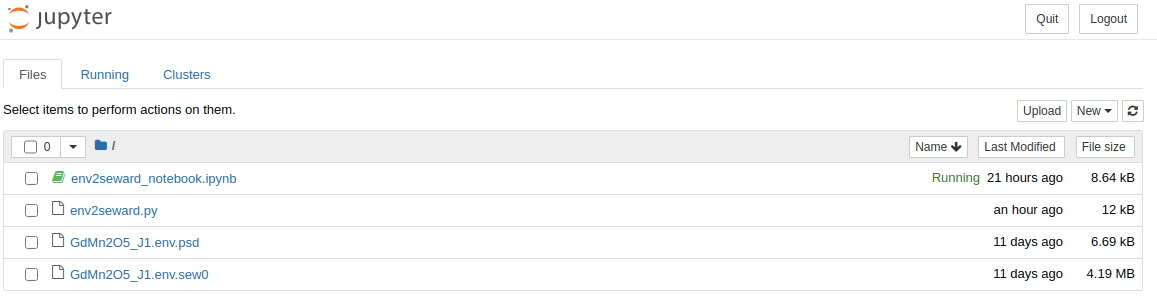
\includegraphics[width=1.3\linewidth]{dashboard.png}
	\caption{Web app dashboard menu}
	\label{fig:screenshot-from-2020-06-23-12-26-13}
\end{figure}

\begin{figure}
	\centering
	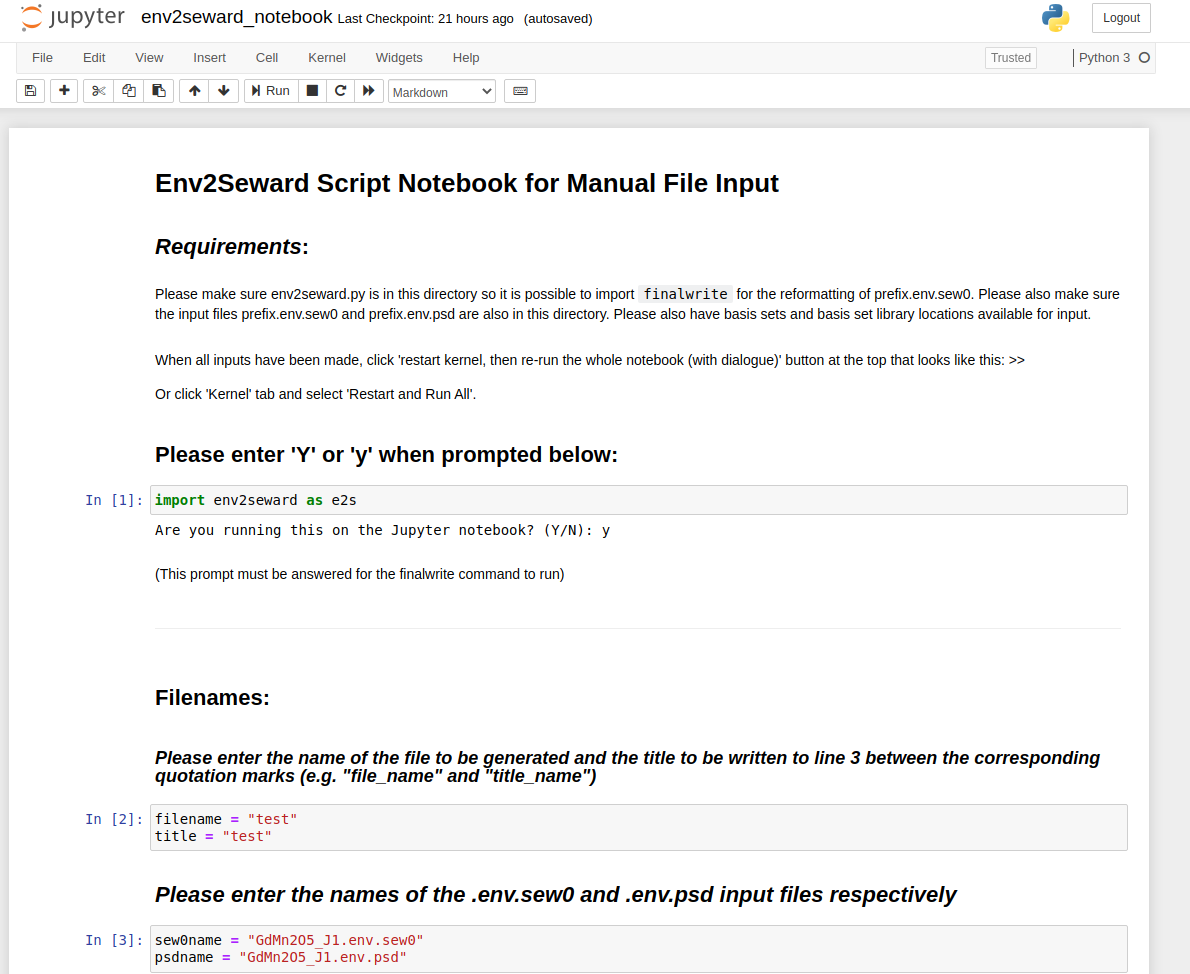
\includegraphics[width=1.3\linewidth]{notebook.png}
	\caption{env2seward\_notebook when opened}
	\label{fig:screenshot-from-2020-06-23-12-26-25}
\end{figure}

In the notebook you will see a page of Jupyter cells, some in markdown (a text formatting language) and some to run python3 code. If you want to learn more about how these work, see \url{https://www.dataquest.io/blog/jupyter-notebook-tutorial/}. In order to run these cells individually, click on them and hit \texttt{Ctrl+Enter} or press the run button (below the cell tab in the toolbar). Please follow the instructions in between the code cells to enter the correct inputs.
If you would like to see the atom-types that require basis set entry, follow the instructions under the subtitle `Basis atoms (see instructions below on how to run this cell):'. The next steps are:

\begin{itemize}
	\item Make sure the inputs have all been entered according to the instructions (filename, title, sew0name, psdname, lib\_frag, lib\_pseudo)
	\item Select the button that says `restart the kernel and re-run the whole notebook' that looks like a fast-forward icon.
	\item If you cannot find this, click the kernel icon (in English, it may be different in other languages), next to cell and widgets, and select `Restart and Run All'.
	\item You will see a prompt in the first code cell (\texttt{import env2seward as e2s}). Please enter `Y'.
	\item After this the last code cell (\texttt{e2s.finalwrite(filename,...}) will output `File has been created' which means you now have a seward input file ready in the webapp directory. You can download this to a specific directory by going back to the dashboard menu, ticking the box next to `\texttt{chosen filename}' and clicking `Download'.
	\item The output file will also naturally appear in the same directory as your \texttt{env2seward\_notebook.ipynb} file.
\end{itemize}

%The section below was throwing up errors so I commented it for later

%&SEWARD
%Title
%GdMn2O5_Pbam -J1
%
%Expert
%Verbose
%
%Basis set
%Mn.ano-rcc.Roos.21s15p10d6f4g2h.6s4p3d1f0g.
%spherical
%Mn01       0.000000000000       0.000000000000       2.749761859316        Bohr
%Mn02       0.000000000000       0.000000000000      -2.749761859316        Bohr
%End of basis
%****
%Basis set
%O.ano-rcc.Roos.14s9p4d3f2g.4s3p1d0f
%spherical
%O203       2.231731397024      -0.875526023191       0.000000000000        Bohr
%O204      -2.231731397024       0.875526023191       0.000000000000        Bohr
%O305       2.118901193775      -1.064763543958      -5.367483621542        Bohr
%O306      -2.118901193775       1.064763543958      -5.367483621542        Bohr
%O407       1.412183935493       3.326902091439      -2.642519536557        Bohr
%O408       1.412183935493       3.326902091439       2.642519536557        Bohr
%O409      -1.412183935493      -3.326902091439       2.642519536557        Bohr
%O410      -1.412183935493      -3.326902091439      -2.642519536557        Bohr
%O311       2.118901193775      -1.064763543958       5.367483621542        Bohr
%O312      -2.118901193775       1.064763543958       5.367483621542        Bohr
%End of basis
%****
%*** Pseudos ***************************************************
%Basis Set
%Gd.ECP.Marie.0s.0s.0e-Gd-GdMn2O5.    / PSEUDO
%pseudocharge
%Gd13       1.944292285644      -5.292197469090       0.000000000000        Bohr
%Gd14      -1.944292285644       5.292197469090       0.000000000000        Bohr
%Gd15       5.003380328217       2.774193015439       0.000000000000        Bohr
%Gd16      -5.003380328217      -2.774193015439       0.000000000000        Bohr
%Gd33      -8.891964899504       2.774193015439       0.000000000000        Bohr
%Gd36       1.944292285644      -5.292197469090     -10.734967243083        Bohr
%Gd37      -1.944292285644       5.292197469090     -10.734967243083        Bohr
%Gd46       1.944292285644      -5.292197469090      10.734967243083        Bohr
%Gd47      -1.944292285644       5.292197469090      10.734967243083        Bohr
%Gd65       8.891964899504      -2.774193015439       0.000000000000        Bohr
%End of Basis
%*
%Basis Set
%Mn.ECP.Marie.0s.0s.0e-Mn1-GdMn2O5.    / PSEUDO
%pseudocharge
%Mn38       0.000000000000       0.000000000000      -7.985205383768        Bohr
%Mn48       0.000000000000       0.000000000000       7.985205383768        Bohr
%End of Basis
%*
%\end{verbatim}

\bibliographystyle{unsrt}
\bibliography{manualbib.bib}
\end{document}
